Although this is called the intro, I've also but int bits that I want to put in that are general for more than one chapter. These need to be sorted eventually...

\section{Statistical Ecology}

Some general remarks about stat ecol perhaps.

\section{Themes}

\bi
	\item Morphing
	\item Modifying penalties
	\item Computational efficiency
	\item Realistic physical models!!!!!!
\ei


\section{Some notational conventions}



\section{Generalized Additive Models}

General GAM setup

\bi
\item Splines
\item objective function
\label{GAMobjfcn}
\item penalties
\label{GAMpenalties}
\item bases - TPRS (and maybe P-splines?)
\item fitting - GCV REML etc
\item other stuff
	\bi
	\item MSE
	\begin{equation}
\text{MSE}(\hat{f}) = \frac{1}{P} \sum_{j=1}^P (\hat{f}(x_j) - z_j)^2,
\end{equation}
the mean difference between the model ($\hat{f}$) evaluated at the prediction points ($\{x_j : j=1 \dots P\}$) and the true value of the function ($\{z_j : j=1 \dots P\}$.) This gives the MSE per model, since here many realisations are run, the mean of these over all simulations is taken and the standard error is calculated.
	\item EDF
	
The estimated degrees of freedom gives an measure of the complexity of the model that was fit to the data. The higher the EDF, the more basis functions were used and  the more complex the model.  Since the models used here are penalised, it is the penalty term that controls the overall ``wigglyness'' of the spline and hence the EDF. Although the basis dimension is set in the model, this is just an upper bound, the smoothing penalty suppresses parts of the model. Therefore basis dimension is not a major concern provided that it is not set too low (\cite{simonbook}, p. 161.) 

	\ei
\ei

\section{Finite area smoothing}

\subsection{Overview of finite area smoothing}

Splines are a popular way of performing spatial smoothing in two dimensions. In this context, they are used to fit smooth functions over a geographical region. A typical application of this is in ecological modelling; a response is sought (be it the density of a population or concentration of a chemical) as a function of its spatial coordinates. The function can then be used to perform inference on the population, whether that be an abundance estimate, density map or a more sophisticated inferential goal.

% leakage example 
\begin{figure}
\centering
% trim order l b r t
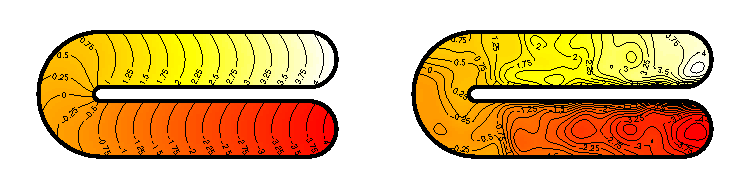
\includegraphics{intro/figs/ramsay-leak.pdf}\\
\caption{An example of leakage. A thin plate regression spline was fit to data sampled from the function on the left, here the model smooths across the gap in the middle of the domain (right.)}
\label{leakage}
\end{figure}

When the geographical region has a \emph{complex boundary}, features from one part of the domain can unduly influence other parts. Considering the boundary as a polygon, a complex boundary is a non-convex polygon, in particular when the non-convexity is relatively extreme. Often this consists of having some peninsula-like feature(s) in the domain with notably different observation values on either side of the feature. Given that there is some scientific motivation as to why those parts of the domain should not affect each other, features such as peninsulae give rise to a phenomenon known as \emph{leakage}; a typical example can be seen in \fig{leakage}. Leakage is the unwanted contamination of one region of an estimated function with those values from another part of the estimated function.

Leakage is problematic since it causes the fitted surface to be mis-estimated; this can then lead to incorrect inference (eg. incorrect abundance estimates), which is clearly not desirable. This can be seen in \fig{leakage} where the high values in the upper part of the domain leak across the gap to the lower values below and vice versa.

The problem of leakage arises because of the way in which the smoother defines how near objects are. Most smoothing techniques use the Euclidean metric to measure the distance between data. Clearly though, this approach is a bad idea: biological populations do not conform to Euclidean geometry in their movement patterns. Just as whales no not uniformly distribute themselves across sea and glacier, domesticated sheep do not spend a lot of time in the middle of the M4. Natural and man made barriers carve up the landscape (and seascape), segregating populations.

The distribution of the population is smooth, just not over $\mathbb{R}^2$ (\cite{wangranalli}.) Instead the structure of the domain that is under investigation must be taken into account and, the appropriate technique used to draw inference.

\subsection{Ramsay's horseshoe function as a benchmark for finite area smoothing}

\cite{ramsay} proposes a function which can be used to benchmark new approaches to 2-dimensional smoothing. The function takes the form of a horseshoe shape which is flat across the domain has a gradient along the domain's major axis. This can be seen in \fig{orig-fs}. \cite{soap} modifies the shape by adding curvature across the minor axis of the shape. This was added in order to avoid the horseshoe function lying in the nullspace of the soap film's penalty, making the problem trivial for a soap film smoother. This second shape shall be referred to as the \emph{Ramsay horseshoe} throughout and is shown in \fig{leakage}.

% original horseshoe from Ramsay's paper
\begin{figure}
\centering
% trim order l b r t
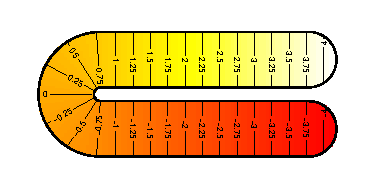
\includegraphics{intro/figs/orig-fs.pdf}\\
\caption{The horseshoe function as it appeared in \cite{ramsay}.}
\label{orig-fs}
\end{figure}

The test function highlights a common problem in spatial smoothing: that of leakage. When the problem is specified in Euclidean distance, the model thinks that the distance between the two arms of the horseshoe is the distance over the gap in between them, rather than the distance along the major axis of the shape. This causes the high function values from one side to contaminate the other (or the low to contaminate the high.) It is easy to see that this causes the smooth to be calculated incorrectly.


		
\subsection{Previous approaches}

The cause of leakage can be characterised in two ways: either the smooth does not respect the boundary of the domain, or the smooth does not take into account the geometry of the domain; in particular with regard to the distance between points within the domain. Previous work in this area has been to combat leakage along these two lines. Work of \cite{ramsay} and \cite{soap} both use a PDE boundary condition approach to try to prevent leakage, where as \cite{wangranalli} and \cite{eilerstalk}  attempt to approximate the intrinsic structure of the domain while not treating the boundary a something special in the basis setup. Here I will be adopting the the latter approach.

The four main works on the topic may be summarised as follows:

\begin{enumerate}
\item \cite{ramsay} proposes finite element $L$-splines (FELSPLINEs.) The $L$-spline has a differential operator in its penalty, which cannot be analytically solved in two dimensions. However, to combat this, the author triangulates the domain and then constructs a set of bivariate quadratic polynomial basis functions over each triangle, specifying that there be continuity over the edges of the triangles. The union of these functions is then a solution to the PDE in the penalty and therefore the solution to the usual smoothing objective function (see \secref{GAMobjfcn}.)

Although FELSPLINE does not exhibit leakage on the horseshoe, in practice it make unrealistic assumptions about the model it fits. The boundary conditions of FELSPLINE specify that the gradient is normal to the boundary at every point, this is not always physically realistic and as \cite{soap} showed, merely by adding a small amount of curvature to the gradient of the Ramsay horseshoe, the method's performance begins to falter.

\item \cite{wangranalli} adopt a ``within-area distance'' formulation for thin plate splines. In this case they take the geodesic distance between two points, that being the shortest path within the domain. This gives a definition of how near objects are in the domain.

Wang and Ranalli approximate the geodesic distance in order to calculate the shortest path. For this they create a weighted, undirected graph, $G$ with datum at each vertex and the distance between each pair of vertices as the weights on the edges. Floyd's algorithm is then used to find the $k$ nearest neighbours of each vertex, they then take the restricted graph of $G$, $G_k$ in which each vertex is only connected to its $k$ nearest neighbours. With this new, restricted, graph the geodesic distances between each pair of vertices can be calculated using Floyds algorithm.

As the author point out, the quality of the approximation is dependent on the size of the data set and its density. At low densities the estimated geodesic distance will tend towards the Euclidean, at high densities the approximation tends, asymptotically toward the true geodesic distance (\cite{bernstein}.)Even with dense data, Floyd's algorithm is cubic in the number of vertices (in this case the size of the data set) so the procedure will be rather slow. Although the $k$-nearest neighbours algorithm used is not specified in the paper SAY SOMETHING MORE HERE!!!!

\item \cite{soap} consider constructing a soap film over the domain. The film is then weighed down by the data, the objective is then to minimize the surface tension in the film. The domain is bounded by some polygon with known or estimated boundary conditions.

Mathematically, the soap film smoother is constructed by first specifying a set of functions $\rho_k(x,y)$, which are each solutions to the Laplace equation in two dimensions:
\be
\frac{\partial^2\rho}{\partial x^2} + \frac{\partial^2\rho}{\partial y^2} = 0
\ee
except at one of the knots ($x^*_k,y^*_k$). Then, solving Poisson's equation in 2-dimensions:
\be
\frac{\partial^2 g_k}{\partial x^2} + \frac{\partial^2 g_k}{\partial y^2} = \rho
\ee
with $\rho=\rho_i(x,y)$, where $i$ indexes the data, the set of basis functions for the soap fiim smoother, $g_k(x,y)$ is found. These bases are then summed to form $f$ the soap film smoother. The standard thin plate spline penalty (\secref{GAMpenalties}) is modified to be:
\be
\int_\Omega \Big(\frac{\partial^2 f}{\partial x^2}+\frac{\partial^2 f}{\partial y^2} \Big)^2,\text{d}x\text{d}y,
\ee
where $\Omega$ is the domain in question and the squaring of the whole integrand rather than each term individually allows the $x$ and $y$ terms to be traded off against each other such that the nullspace of the penalty is infinite dimensional. This allows those functions in the nullspace to be sufficiently wiggly to meet any boundary conditions.

The solution of the PDEs above, giving the basis and penalty is the most computationally expensive part of the procedure. Knots to use for $x_k^*$ and $y_k^*$ must be specified and although a grid is usually used, numerical problems occur when knots are placed in boundary cells in the PDE solution grid.

\item An alternative approach is to morph the points within the domain to instead lie in a domain which is more suitable for smoothing. For example, with Ramsay's horseshoe, it seems intuitive to simply bend the horseshoe into a long strip and then smooth on that domain. Indeed, \cite{eilerstalk} proposed using the \sch transform for this very purpose (I, independently, came to this method via my obsessive listening to BBC Radio 4.)

Creating some kind of mapping between the space in which the data lies and the space in which conventional smoothers perform well has a lot of promise. Not having to setup a new basis structure and relying on long tested methodology is clearly appealing.

\end{enumerate}

\section{Distance sampling}

This will be a very brief introduction to distance sampling methods, in the style of the encyclopaedia of environmetrics article.
